\documentclass[11pt,a4paper]{article}

\usepackage[utf8]{inputenc}
\usepackage[T1]{fontenc}
\usepackage{geometry}
\usepackage{graphicx}
\usepackage{booktabs}
\usepackage{longtable}
\usepackage{array}
\usepackage{xcolor}
\usepackage{listings}
\usepackage{tikz}
\usepackage{hyperref}
\usepackage{fancyhdr}
\usepackage{titlesec}
\usepackage{enumitem}
\usepackage{caption}
\usepackage{amsmath}
\usepackage{float}
\usepackage{inconsolata}  % Better monospace font for code

\geometry{margin=1in}

% Define colors
\definecolor{headerblue}{RGB}{0,82,147}
\definecolor{lightgray}{RGB}{245,245,245}
\definecolor{codegray}{RGB}{240,240,240}

% Listings configuration for 6502 assembly
\lstdefinelanguage{asm6502}{
    morekeywords={lda,ldx,ldy,sta,stx,sty,tax,tay,txa,tya,tsx,txs,pha,pla,php,plp,
                  and,ora,eor,adc,sbc,cmp,cpx,cpy,inc,inx,iny,dec,dex,dey,
                  asl,lsr,rol,ror,jmp,jsr,rts,rti,bcc,bcs,beq,bne,bmi,bpl,bvc,bvs,
                  clc,sec,cli,sei,clv,cld,sed,nop,brk},
    sensitive=false,
    morecomment=[l]{;},
    morestring=[b]",
}

\lstset{
    basicstyle=\ttfamily\small,
    backgroundcolor=\color{codegray},
    frame=single,
    breaklines=true,
    captionpos=b,
}

% Header/Footer
\pagestyle{fancy}
\fancyhf{}
\fancyhead[L]{\textbf{6502 Microcontroller}}
\fancyhead[R]{Datasheet v1.0}
\fancyfoot[C]{\thepage}

% Title formatting
\titleformat{\section}
    {\Large\bfseries\color{headerblue}}
    {\thesection}{1em}{}
\titleformat{\subsection}
    {\large\bfseries\color{headerblue}}
    {\thesubsection}{1em}{}

\begin{document}

% Title Page
\begin{titlepage}
    \centering
    \vspace*{2cm}
    {\Huge\bfseries\color{headerblue} 6502 Microcontroller\\[0.5cm]}
    {\Large Complete CPU with Bus Multiplexer\\[0.3cm]}
    {\large GPIO, Timer, and UART Controller\\[2cm]}

    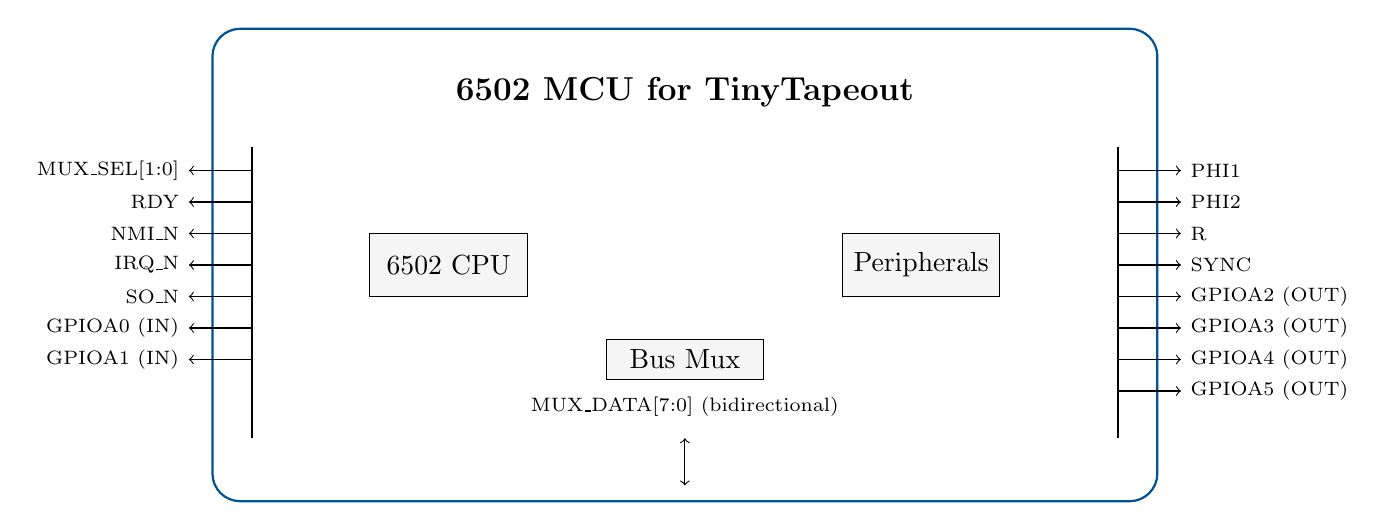
\begin{tikzpicture}
        \draw[thick, headerblue, rounded corners=10pt] (0,0) rectangle (12,6);
        \node at (6,5.2) {\large\textbf{6502 MCU for TinyTapeout}};

        % Left side - inputs
        \draw[thick] (0.5,0.8) -- (0.5,4.5);
        \foreach \y/\txt in {4.2/MUX\_SEL[1:0], 3.8/RDY, 3.4/NMI\_N, 3.0/IRQ\_N, 2.6/SO\_N, 2.2/GPIOA0 (IN), 1.8/GPIOA1 (IN)} {
            \draw[<-] (-0.3,\y) -- (0.5,\y);
            \node[left, font=\scriptsize] at (-0.3,\y) {\txt};
        }

        % Right side - outputs
        \draw[thick] (11.5,0.8) -- (11.5,4.5);
        \foreach \y/\txt in {4.2/PHI1, 3.8/PHI2, 3.4/R/W, 3.0/SYNC, 2.6/GPIOA2 (OUT), 2.2/GPIOA3 (OUT), 1.8/GPIOA4 (OUT), 1.4/GPIOA5 (OUT)} {
            \draw[->] (11.5,\y) -- (12.3,\y);
            \node[right, font=\scriptsize] at (12.3,\y) {\txt};
        }

        % Bottom - bidirectional
        \node at (6,1.2) {\scriptsize MUX\_DATA[7:0] (bidirectional)};
        \draw[<->] (6,0.8) -- (6,0.2);

        % Internal blocks
        \node[draw, rectangle, fill=lightgray, minimum width=2cm, minimum height=0.8cm] at (3,3) {6502 CPU};
        \node[draw, rectangle, fill=lightgray, minimum width=2cm, minimum height=0.8cm] at (9,3) {Peripherals};
        \node[draw, rectangle, fill=lightgray, minimum width=2cm, minimum height=0.5cm] at (6,1.8) {Bus Mux};
    \end{tikzpicture}

    \vfill
    {\large Technical Datasheet\\[0.5cm]}
    {\normalsize Document Version 1.0\\}
    {\normalsize\today}
\end{titlepage}

\tableofcontents
\newpage

%==============================================================================
\section{Overview}
%==============================================================================

The TinyTapeout 6502 Microcontroller is a complete MOS Technology 6502-compatible CPU with integrated peripherals, designed specifically for the TinyTapeout platform. This implementation features a bus multiplexer architecture that efficiently uses the limited 24-pin interface to expose the full CPU bus and peripheral functions.

\subsection{Key Features}

\begin{itemize}[leftmargin=*]
    \item \textbf{Complete 6502 CPU}: Cycle-accurate implementation with all documented opcodes
    \item \textbf{Bus Multiplexer}: 4-phase multiplexing reduces pin count from 24 to 8 data pins
    \item \textbf{External Memory Support}: Up to 64KB address space via multiplexed bus
    \item \textbf{Integrated Peripherals}:
        \begin{itemize}
            \item GPIO: 6 pins (2 input-only, 4 output-only on TinyTapeout; internally bidirectional)
            \item UART: 8N1 serial with 4-byte TX/RX FIFOs
            \item Timer: 16-bit timer with prescaler and interrupt support
            \item Clock Control: Runtime CPU clock division
        \end{itemize}
    \item \textbf{Pin Multiplexing}: UART and GPIO can share physical pins via mode registers
    \item \textbf{TinyTapeout Optimized}: Fits in 2×2 tile allocation with efficient gate usage
\end{itemize}

\subsection{Target Applications}

\begin{itemize}[leftmargin=*]
    \item Educational 6502 system on a chip
    \item Retro computing demonstrations
    \item LED display controllers with programmability
    \item Serial communication nodes
    \item Embedded control applications
\end{itemize}

\subsection{Implementation Details}

\begin{itemize}[leftmargin=*]
    \item \textbf{RTL Size}: ~2,900 lines of SystemVerilog
    \item \textbf{Technology}: IHP SG13G2 130nm
    \item \textbf{Die Size}: 2×2 TinyTapeout tiles (419.52µm × 313.74µm)
    \item \textbf{Clock}: 50 MHz nominal (configurable)
    \item \textbf{CPU Speed}: Software-configurable from full speed down to 1/256× via clock divider
\end{itemize}

%==============================================================================
\section{System Architecture}
%==============================================================================

\subsection{Block Diagram}

The system consists of three major components:

\begin{enumerate}
    \item \textbf{6502 CPU Core}: Executes instructions and drives the internal bus
    \item \textbf{Bus Multiplexer}: Converts 16-bit address + 8-bit data to 8-bit multiplexed bus
    \item \textbf{Memory-Mapped Peripherals}: GPIO, UART, Timer, Clock Control
\end{enumerate}

The CPU accesses both internal peripherals and external memory through a unified 64KB address space. Address decoding logic routes accesses to 0xA000-0xA047 to internal peripherals, while all other addresses are multiplexed to the external bus.

\subsection{Memory Map}

\begin{table}[H]
\centering
\begin{tabular}{lll}
\toprule
\textbf{Address Range} & \textbf{Size} & \textbf{Description} \\
\midrule
0x0000 -- 0x9FFF & 40KB & External memory (via bus mux) \\
0xA000 -- 0xA00B & 12 bytes & GPIO registers \\
0xA010 -- 0xA017 & 8 bytes & Reserved \\
0xA020 -- 0xA027 & 8 bytes & Timer \\
0xA030 -- 0xA033 & 4 bytes & Clock control \\
0xA040 -- 0xA047 & 8 bytes & UART \\
0xA048 -- 0xFFFF & ~22KB & External memory (via bus mux) \\
\bottomrule
\end{tabular}
\caption{System Memory Map}
\end{table}

Typical usage allocates external RAM at 0x0000-0x7FFF and ROM at 0x8000-0xFFFF, with the 6502 reset vector at 0xFFFC pointing to boot code.

\subsection{Bus Multiplexer Protocol}

The bus multiplexer reduces pin requirements by time-multiplexing the address and data buses over 8 shared bidirectional pins. The external controller (e.g., RP2040 on TinyTapeout demo board) sequences through 4 phases within each CPU cycle:

\begin{table}[H]
\centering
\begin{tabular}{clll}
\toprule
\textbf{MUX\_SEL} & \textbf{Phase} & \textbf{Direction} & \textbf{Data on Bus} \\
\midrule
01 & ADDR\_HI & MCU → External & Address[15:8] \\
00 & ADDR\_LO & MCU → External & Address[7:0] \\
10 & DATA\_IN & External → MCU & Read data (if R/W=1) \\
11 & DATA\_OUT & MCU → External & Write data (if R/W=0) \\
\bottomrule
\end{tabular}
\caption{Bus Multiplexer Phases}
\end{table}

All four phases complete within a single 6502 bus cycle, so there is \textbf{no performance penalty} compared to a parallel bus. The external controller monitors PHI2 to track cycle boundaries and controls MUX\_SEL accordingly.

%==============================================================================
\section{Pin Configuration}
%==============================================================================

The TinyTapeout interface provides 24 pins total: 8 dedicated inputs (ui\_in), 8 dedicated outputs (uo\_out), and 8 bidirectional pins (uio). This implementation uses all available pins efficiently:

\subsection{Input Pins (ui\_in[7:0])}

\begin{table}[H]
\centering
\begin{tabular}{ll}
\toprule
\textbf{Pin} & \textbf{Function} \\
\midrule
ui\_in[0] & MUX\_SEL[0] -- Bus phase select bit 0 \\
ui\_in[1] & MUX\_SEL[1] -- Bus phase select bit 1 \\
ui\_in[2] & RDY -- CPU ready signal (active high) \\
ui\_in[3] & NMI\_N -- Non-maskable interrupt (active low) \\
ui\_in[4] & IRQ\_N -- Interrupt request (active low) \\
ui\_in[5] & SO\_N -- Set overflow flag (active low) \\
ui\_in[6] & GPIOA0 -- GPIO pin 0 input (unidirectional) \\
ui\_in[7] & GPIOA1 -- GPIO pin 1 input (unidirectional) \\
\bottomrule
\end{tabular}
\caption{Input Pin Assignments}
\end{table}

\subsection{Output Pins (uo\_out[7:0])}

\begin{table}[H]
\centering
\begin{tabular}{ll}
\toprule
\textbf{Pin} & \textbf{Function} \\
\midrule
uo\_out[0] & PHI1 -- CPU phase 1 clock \\
uo\_out[1] & PHI2 -- CPU phase 2 clock \\
uo\_out[2] & R/W -- Read/write signal (1=read, 0=write) \\
uo\_out[3] & SYNC -- Opcode fetch indicator \\
uo\_out[4] & GPIOA2 -- GPIO pin 2 output (unidirectional) \\
uo\_out[5] & GPIOA3 -- GPIO pin 3 output (unidirectional) \\
uo\_out[6] & GPIOA4 -- GPIO pin 4 output (unidirectional) \\
uo\_out[7] & GPIOA5 -- GPIO pin 5 output (unidirectional) \\
\bottomrule
\end{tabular}
\caption{Output Pin Assignments}
\end{table}

\subsection{Bidirectional Pins (uio[7:0])}

\begin{table}[H]
\centering
\begin{tabular}{ll}
\toprule
\textbf{Pin} & \textbf{Function} \\
\midrule
uio[7:0] & MUX\_DATA[7:0] -- Multiplexed address/data bus \\
\bottomrule
\end{tabular}
\caption{Bidirectional Pin Assignments}
\end{table}

The MUX\_DATA pins are driven by the MCU during ADDR\_HI, ADDR\_LO, and DATA\_OUT phases, and tri-stated during DATA\_IN phase to allow the external controller to drive read data.

\subsection{GPIO Pin Mapping}

While the MCU's internal GPIO peripheral is fully bidirectional, the TinyTapeout pin assignment splits GPIO across input and output pins:

\begin{itemize}
    \item \textbf{GPIO 0-1}: Input-only (read via INPUT register at 0xA002)
    \item \textbf{GPIO 2-5}: Output-only (write via OUTPUT register at 0xA001, controlled by OE register at 0xA000)
\end{itemize}

Each GPIO pin has an independent mode register (0xA004-0xA009) that can configure it as:
\begin{itemize}
    \item GPIO mode (0x00) -- Standard I/O
    \item UART TX mode (0x01) -- UART transmit output
    \item UART RX mode (0x02) -- UART receive input
\end{itemize}

See Section 4 for complete GPIO peripheral documentation.

%==============================================================================
\section{Peripheral Registers}
%==============================================================================

\subsection{GPIO Peripheral (0xA000-0xA00B)}

\subsubsection{Register Map}

\begin{longtable}{lll}
\toprule
\textbf{Address} & \textbf{Register} & \textbf{Description} \\
\midrule
\endhead
0xA000 & OE & Output Enable (0=input, 1=output) \\
0xA001 & OUT & Output Data \\
0xA002 & IN & Input Data (read-only) \\
0xA003 & Reserved & -- \\
0xA004 & MODE\_PIN0 & Pin 0 function select \\
0xA005 & MODE\_PIN1 & Pin 1 function select \\
0xA006 & MODE\_PIN2 & Pin 2 function select \\
0xA007 & MODE\_PIN3 & Pin 3 function select \\
0xA008 & MODE\_PIN4 & Pin 4 function select \\
0xA009 & MODE\_PIN5 & Pin 5 function select \\
0xA00A & MODE\_PIN6 & Reserved (unused) \\
0xA00B & MODE\_PIN7 & Reserved (unused) \\
\bottomrule
\caption{GPIO Register Map}
\end{longtable}

\textbf{Note}: Only GPIO 0-5 are connected to TinyTapeout pins. GPIO 6-7 registers exist but are not connected.

\subsubsection{Pin Mode Values}

\begin{table}[H]
\centering
\begin{tabular}{ll}
\toprule
\textbf{Value} & \textbf{Function} \\
\midrule
0x00 & GPIO -- Standard I/O controlled by OE/OUT \\
0x01 & UART0\_TX -- UART transmit output \\
0x02 & UART0\_RX -- UART receive input \\
0x03-0xFF & Reserved \\
\bottomrule
\end{tabular}
\caption{GPIO Pin Mode Values}
\end{table}

\subsubsection{Example: Configuring GPIO}

\begin{lstlisting}[language=asm6502, caption=Configure GPIO pins]
; Set GPIO2 as output, GPIO3 as output
LDA #$0C          ; Bits 2 and 3
STA $A000         ; Write to OE register

; Set GPIO2 high, GPIO3 low
LDA #$04          ; Bit 2
STA $A001         ; Write to OUT register

; Read GPIO0 and GPIO1
LDA $A002         ; Read IN register
AND #$03          ; Mask bits 0-1
\end{lstlisting}

\subsubsection{Example: Configuring UART on GPIO}

\begin{lstlisting}[language=asm6502, caption=Configure UART TX on GPIO2 and RX on GPIO3]
; Set GPIO2 as UART TX
LDA #$01          ; UART0_TX mode
STA $A006         ; MODE_PIN2

; Set GPIO3 as UART RX
LDA #$02          ; UART0_RX mode
STA $A007         ; MODE_PIN3
\end{lstlisting}

\subsection{Timer (0xA020-0xA027)}

16-bit up-counter with prescaler, auto-reload, and interrupt support.

\subsubsection{Register Map}

\begin{longtable}{lll}
\toprule
\textbf{Address} & \textbf{Register} & \textbf{Description} \\
\midrule
\endhead
0xA020 & CTRL & Control register \\
0xA021 & STATUS & Status register (bit 0 = OVERFLOW) \\
0xA022 & COUNT\_LO & Counter low byte (read-only) \\
0xA023 & COUNT\_HI & Counter high byte (read-only) \\
0xA024 & RELOAD\_LO & Reload value low byte \\
0xA025 & RELOAD\_HI & Reload value high byte \\
0xA026 & PRESCALER & Clock prescaler (0-255) \\
0xA027 & Reserved & -- \\
\bottomrule
\caption{Timer Register Map}
\end{longtable}

\subsubsection{Control Register (CTRL)}

\begin{itemize}
    \item Bit 0: ENABLE -- Enable timer counting
    \item Bit 1: AUTO\_RELOAD -- Reload from RELOAD\_LO/HI on overflow
    \item Bit 2: IRQ\_ENABLE -- Enable interrupt on overflow
    \item Bit 3: LOAD -- Load counter from reload registers (write-only strobe, only works when ENABLE=0)
    \item Bits 7-4: Reserved
\end{itemize}

\subsubsection{Example: Periodic Timer with Polling}

\begin{lstlisting}[language=asm6502, caption=1ms periodic timer at 50MHz]
; Calculate prescaler for 1ms tick at 50MHz
; Desired: 1000 ticks per second
; Timer freq = 50MHz / (PRESCALER + 1)
; For 50kHz: PRESCALER = 999
; Overflow period = 65536 / 50000 = 1.31s

; Better: PRESCALER = 49 for 1MHz tick rate
; Then set RELOAD to get 1ms period (1000 ticks)

init_timer:
    ; Set prescaler for 1MHz tick
    LDA #49           ; sysclk / 50 = 1MHz
    STA $A026         ; PRESCALER

    ; Set reload for 1000 ticks = 1ms
    ; Reload value = 65536 - 1000 = 64536 = 0xFC18
    LDA #$18
    STA $A024         ; RELOAD_LO
    LDA #$FC
    STA $A025         ; RELOAD_HI

    ; Load counter and enable with auto-reload
    LDA #$08          ; LOAD (timer stopped)
    STA $A020
    LDA #$03          ; ENABLE | AUTO_RELOAD
    STA $A020

timer_loop:
    ; Poll for overflow
    LDA $A021         ; Read STATUS
    AND #$01          ; Check OVERFLOW
    BEQ timer_loop    ; Wait for overflow

    ; Clear overflow flag
    LDA #$01
    STA $A021

    ; Do 1ms periodic work here
    JSR do_work

    JMP timer_loop

do_work:
    ; Your code here
    RTS
\end{lstlisting}

\subsection{Clock Control (0xA030-0xA033)}

Runtime CPU clock division for dynamic frequency scaling.

\subsubsection{Register Map}

\begin{longtable}{lll}
\toprule
\textbf{Address} & \textbf{Register} & \textbf{Description} \\
\midrule
\endhead
0xA030 & CPU\_DIV & CPU clock divisor (0-255) \\
0xA031 & Reserved & -- \\
0xA032 & STATUS & Clock status (bit 0 = CPU\_LOCKED) \\
0xA033 & Reserved & -- \\
\bottomrule
\caption{Clock Control Register Map}
\end{longtable}

\textbf{CPU Clock Formula}: cpu\_freq = cpu\_clk / (CPU\_DIV + 1)

Where cpu\_clk is the hardware-divided clock (configured by CPU\_CLOCK\_HW\_DIV parameter).

\subsubsection{Example: Power Saving}

\begin{lstlisting}[language=asm6502, caption=Slow down CPU while waiting]
; Reduce CPU speed to 1/16 while idle
idle_loop:
    LDA #$0F          ; Divide by 16
    STA $A030         ; CPU_DIV

    ; Poll for event at slower speed
wait_event:
    LDA $A002         ; Read GPIO
    AND #$01          ; Check button
    BEQ wait_event

    ; Restore full speed
    LDA #$00
    STA $A030         ; CPU_DIV = 0 (full speed)

    ; Handle event
    JSR handle_event
    JMP idle_loop
\end{lstlisting}

\subsection{UART (0xA040-0xA047)}

8N1 serial communication with 4-byte TX/RX FIFOs and configurable baud rate.

\subsubsection{Register Map}

\begin{longtable}{lll}
\toprule
\textbf{Address} & \textbf{Register} & \textbf{Description} \\
\midrule
\endhead
0xA040 & CTRL & Control register \\
0xA041 & STATUS & Status register \\
0xA042 & DATA & Data register (FIFO access) \\
0xA043 & BAUD\_LO & Baud divisor low byte \\
0xA044 & BAUD\_HI & Baud divisor high byte \\
0xA045-0xA047 & Reserved & -- \\
\bottomrule
\caption{UART Register Map}
\end{longtable}

\subsubsection{Control Register (CTRL)}

\begin{itemize}
    \item Bit 0: TX\_ENABLE -- Enable transmitter
    \item Bit 1: RX\_ENABLE -- Enable receiver
    \item Bit 2: TX\_IRQ\_EN -- Enable TX ready interrupt
    \item Bit 3: RX\_IRQ\_EN -- Enable RX ready interrupt
    \item Bits 7-4: Reserved
\end{itemize}

\subsubsection{Status Register (STATUS)}

\begin{itemize}
    \item Bit 0: TX\_READY -- TX FIFO not full (can write)
    \item Bit 1: RX\_READY -- RX FIFO not empty (can read)
    \item Bit 2: TX\_EMPTY -- TX FIFO completely empty
    \item Bit 3: RX\_FULL -- RX FIFO full
    \item Bit 4: TX\_ACTIVE -- Currently transmitting
    \item Bit 5: RX\_ERROR -- Framing error detected
    \item Bits 7-6: Reserved
\end{itemize}

\subsubsection{Baud Rate Formula}

baud\_rate = sysclk / (16 × (divisor + 1))

Common baud rates at 50MHz:

\begin{table}[H]
\centering
\begin{tabular}{lll}
\toprule
\textbf{Baud Rate} & \textbf{Divisor} & \textbf{BAUD\_HI:LO} \\
\midrule
9600 & 325 & 0x01:0x45 \\
19200 & 162 & 0x00:0xA2 \\
38400 & 80 & 0x00:0x50 \\
57600 & 53 & 0x00:0x35 \\
115200 & 26 & 0x00:0x1A \\
\bottomrule
\end{tabular}
\caption{Common Baud Rates (50MHz sysclk)}
\end{table}

\subsubsection{Example: UART "Hello World"}

\begin{lstlisting}[language=asm6502, caption=Transmit string via UART]
; Configure GPIO2 as UART TX
LDA #$01          ; UART0_TX mode
STA $A006         ; MODE_PIN2

; Initialize UART for 9600 baud @ 50MHz
init_uart:
    ; Set baud rate (divisor = 325 = 0x0145)
    LDA #$45
    STA $A043         ; BAUD_LO
    LDA #$01
    STA $A044         ; BAUD_HI

    ; Enable TX
    LDA #$01          ; TX_ENABLE
    STA $A040         ; CTRL

; Transmit "Hello\r\n"
send_hello:
    LDX #0
tx_loop:
    LDA message, X
    BEQ tx_done

    ; Wait for TX ready
tx_wait:
    LDA $A041         ; Read STATUS
    AND #$01          ; Check TX_READY
    BEQ tx_wait       ; Wait if FIFO full

    LDA message, X
    STA $A042         ; Write byte
    INX
    BNE tx_loop

tx_done:
    RTS

message:
    .byte "Hello", $0D, $0A, 0  ; CR+LF+null
\end{lstlisting}

%==============================================================================
\section{External Memory Interface}
%==============================================================================

\subsection{Bus Multiplexer Operation}

The external controller (typically an RP2040 on the TinyTapeout demo board) must:

\begin{enumerate}
    \item Monitor PHI2 to detect cycle boundaries
    \item Wait for address setup time (tADS $\\approx$ 150ns after falling PHI2)
    \item Sequence MUX\_SEL through address phases:
        \begin{itemize}
            \item MUX\_SEL = 01 → Latch ADDR[15:8] from MUX\_DATA
            \item MUX\_SEL = 00 → Latch ADDR[7:0] from MUX\_DATA
        \end{itemize}
    \item During PHI2 high, provide or capture data:
        \begin{itemize}
            \item If R/W = 1 (read): Set MUX\_SEL = 10, drive MUX\_DATA with memory contents
            \item If R/W = 0 (write): Set MUX\_SEL = 11, capture MUX\_DATA to memory
        \end{itemize}
\end{enumerate}

All phases complete within one CPU cycle. At 1MHz CPU clock, each phase has approximately 175ns for address and 500ns for data.

\subsection{Timing Diagram}

\begin{figure}[H]
\centering
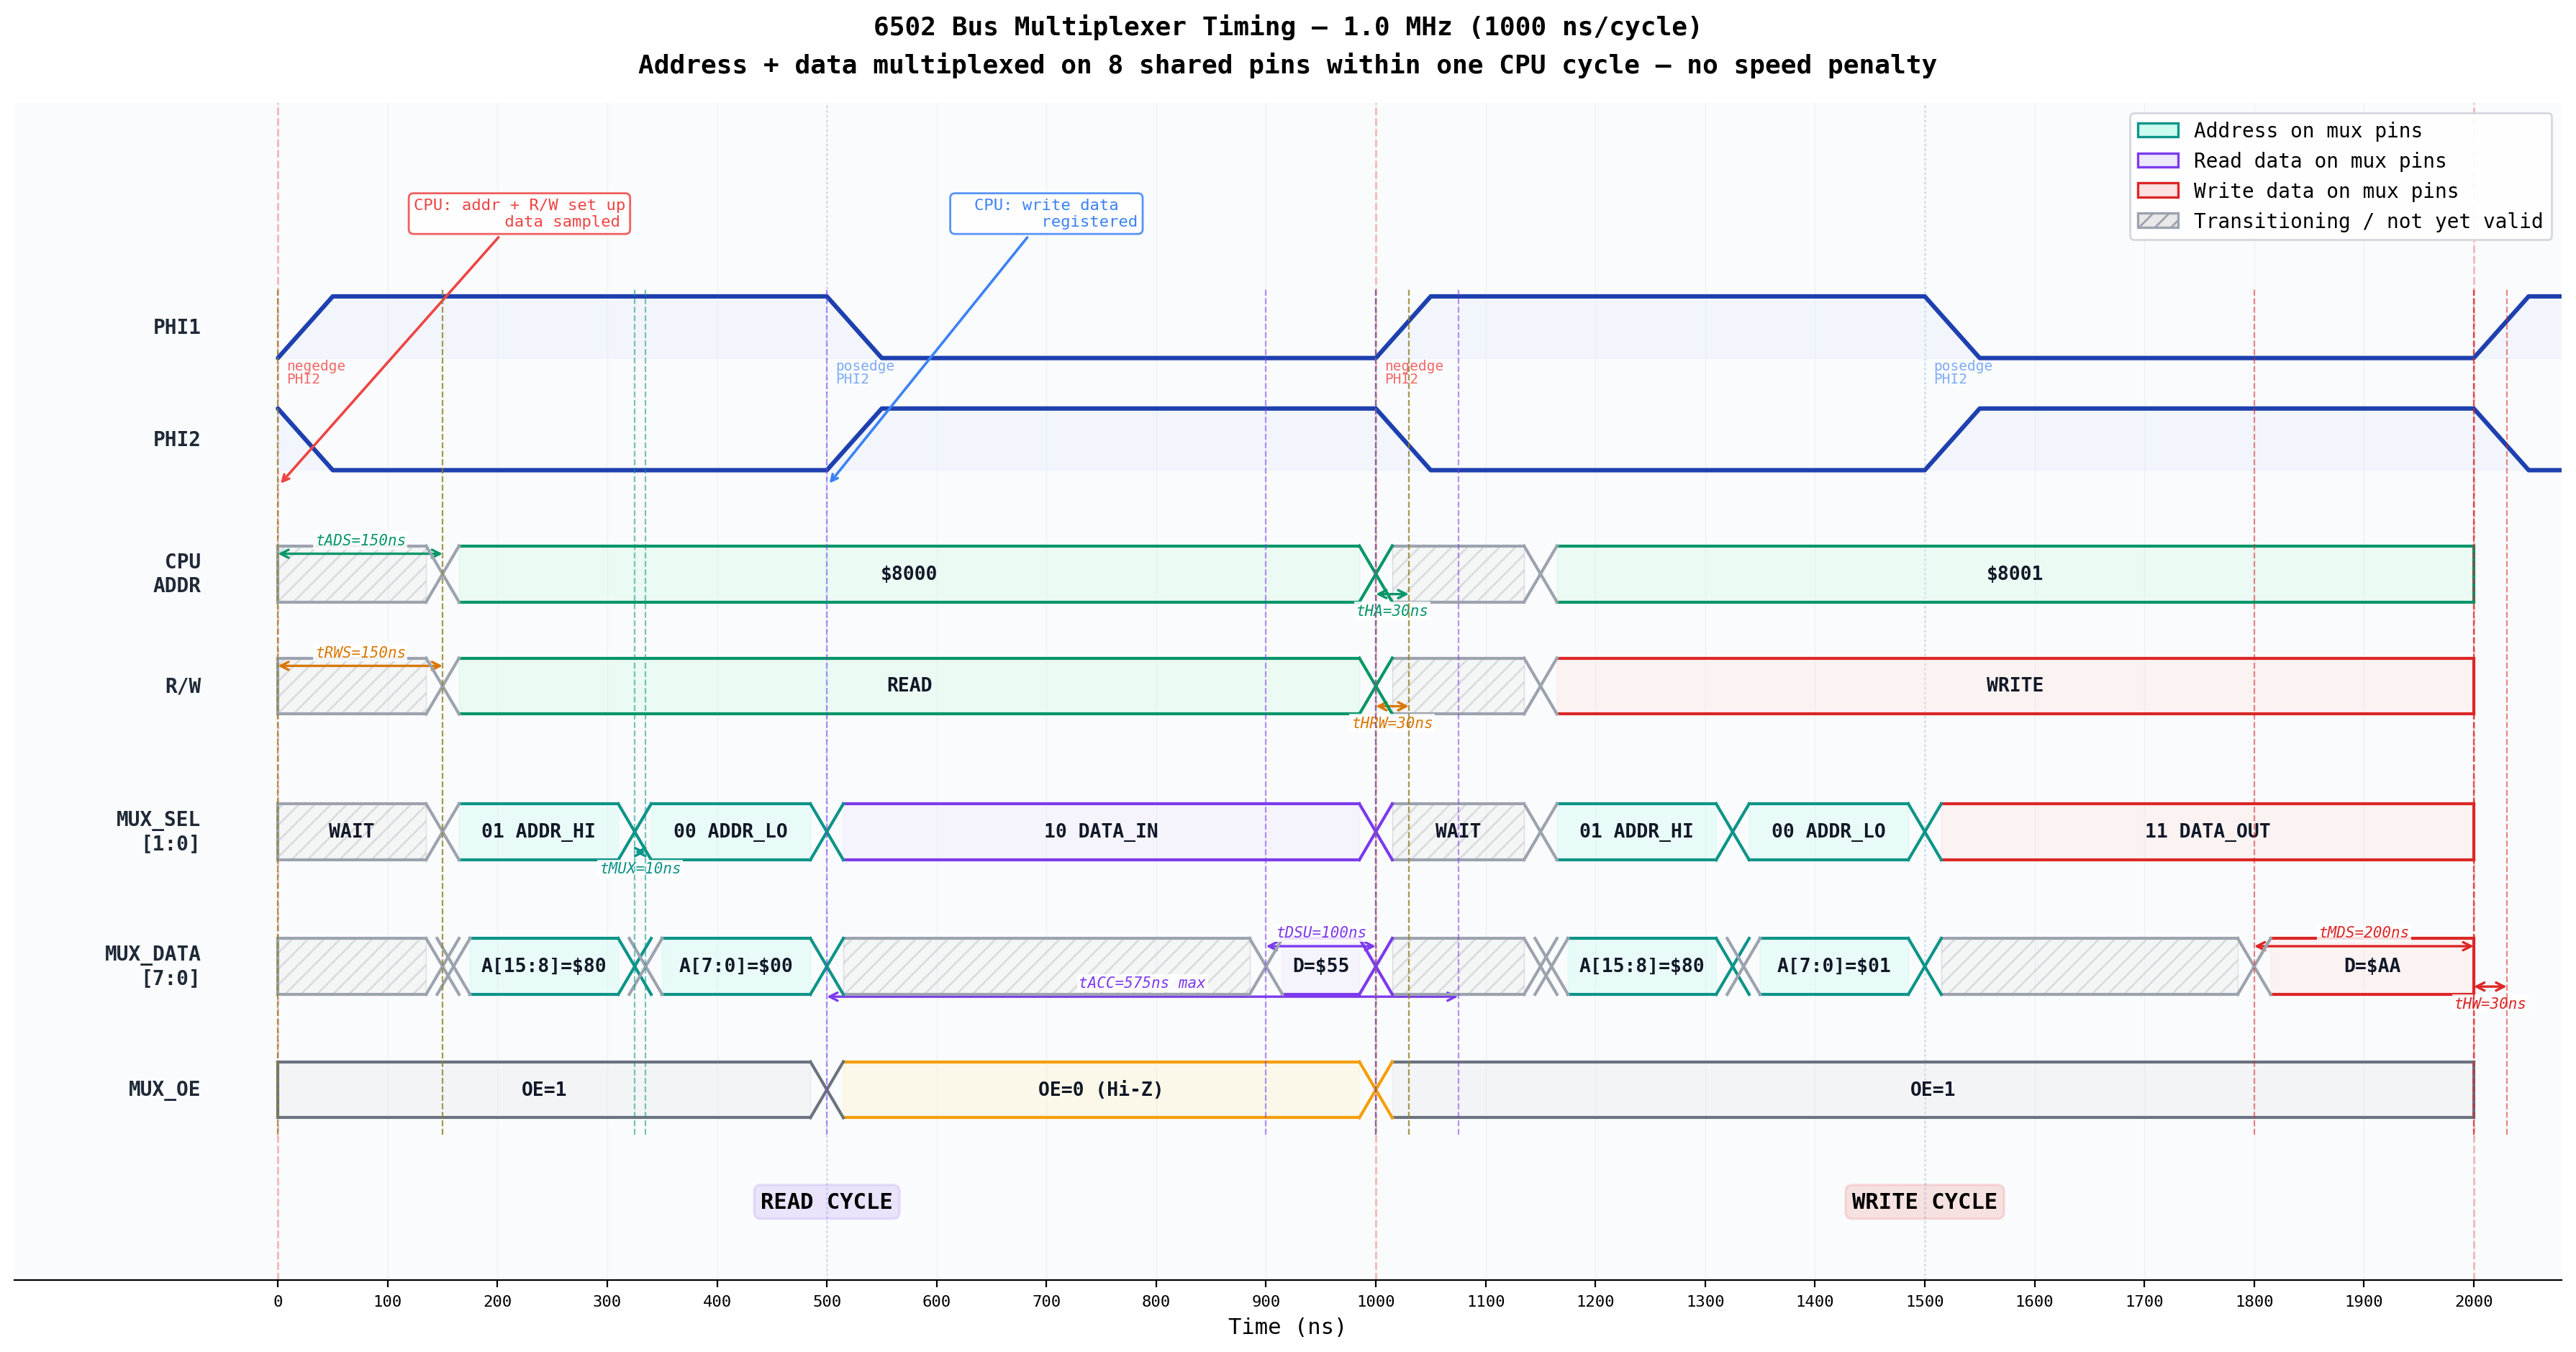
\includegraphics[width=1.0\textwidth]{timing_1mhz.png}
\caption{Bus Multiplexer Timing Diagram (1MHz CPU clock)}
\end{figure}

\subsection{Required External Signals}

The external memory controller needs these signals from the MCU:

\begin{itemize}
    \item \textbf{PHI2} (uo\_out[1]): CPU clock for cycle tracking
    \item \textbf{R/W} (uo\_out[2]): Read (1) or write (0)
    \item \textbf{SYNC} (uo\_out[3]): Optional, indicates opcode fetch
    \item \textbf{MUX\_DATA} (uio[7:0]): Bidirectional multiplexed bus
\end{itemize}

And drives:
\begin{itemize}
    \item \textbf{MUX\_SEL[1:0]} (ui\_in[1:0]): Phase select
    \item \textbf{MUX\_DATA} (uio[7:0]): Drive during read data phase
\end{itemize}

\subsection{RP2040 PIO Example}

The TinyTapeout demo board includes an RP2040 that can serve as the memory controller using its Programmable I/O (PIO) subsystem. A complete reference implementation is available in the upstream m6502 project.

%==============================================================================
\section{Getting Started}
%==============================================================================

\subsection{Minimal System}

A minimal working system requires:

\begin{enumerate}
    \item \textbf{External Memory Controller}: RP2040 or similar
    \item \textbf{Power \& Clock}: 3.3V supply, 50MHz clock
    \item \textbf{Reset}: Active-low reset signal
    \item \textbf{Memory Contents}: ROM image with 6502 code and reset vector
\end{enumerate}

\subsection{Reset Vector}

On reset, the 6502 CPU:
\begin{enumerate}
    \item Loads the program counter from addresses 0xFFFC-0xFFFD (reset vector)
    \item Begins executing code at that address
\end{enumerate}

Ensure your ROM image contains a valid reset vector pointing to your startup code.

\subsection{Example: LED Blink Program}

\begin{lstlisting}[language=asm6502, caption=Simple LED blink on GPIO2]
.org $8000            ; ROM starts at 0x8000

reset:
    ; Configure GPIO2 as output
    LDA #$04          ; Bit 2
    STA $A000         ; OE register

main_loop:
    ; Toggle GPIO2
    LDA $A001         ; Read current output
    EOR #$04          ; Toggle bit 2
    STA $A001         ; Write back

    ; Delay
    JSR delay
    JMP main_loop

delay:
    LDY #$00
delay_outer:
    LDX #$00
delay_inner:
    NOP
    DEX
    BNE delay_inner
    DEY
    BNE delay_outer
    RTS

; Reset vector
.org $FFFC
.word reset           ; Reset vector points to reset routine
.word reset           ; NMI vector (reuse reset for simplicity)
\end{lstlisting}

\subsection{Toolchain}

Common 6502 assemblers and tools:
\begin{itemize}
    \item \textbf{cc65}: C compiler and assembler suite
    \item \textbf{ACME}: Cross-assembler
    \item \textbf{xa65}: Cross-assembler
    \item \textbf{py65}: Python-based 6502 simulator for testing
\end{itemize}

%==============================================================================
\section{Specifications}
%==============================================================================

\subsection{Electrical Characteristics}

\begin{table}[H]
\centering
\begin{tabular}{llll}
\toprule
\textbf{Parameter} & \textbf{Min} & \textbf{Typ} & \textbf{Max} \\
\midrule
Supply Voltage & 1.1V & 1.2V & 1.3V \\
I/O Voltage & 3.0V & 3.3V & 3.6V \\
Clock Frequency & DC & 50MHz & 100MHz \\
Power Consumption & -- & TBD & TBD \\
\bottomrule
\end{tabular}
\caption{Electrical Characteristics}
\end{table}

\subsection{Timing Specifications}

At 50MHz system clock:

\begin{table}[H]
\centering
\begin{tabular}{lll}
\toprule
\textbf{Parameter} & \textbf{Value} & \textbf{Notes} \\
\midrule
CPU Clock (default) & 50MHz & Configurable via CPU\_CLOCK\_HW\_DIV \\
CPU Clock (min) & 195kHz & CPU\_DIV = 255 \\
UART Baud Rate & 9600-115200 & Standard rates supported \\
Timer Resolution & 20ns & At 50MHz sysclk, PRESCALER=0 \\
\bottomrule
\end{tabular}
\caption{Timing Specifications}
\end{table}

\subsection{Resource Utilization}

Estimated gate count breakdown (2×2 TinyTapeout tiles):

\begin{table}[H]
\centering
\begin{tabular}{ll}
\toprule
\textbf{Component} & \textbf{Approximate Lines} \\
\midrule
6502 CPU Core & 923 \\
Bus Multiplexer & 44 \\
GPIO Peripheral & 135 \\
UART (TX+RX+Main) & 472 \\
Timer & 151 \\
Clock Control & 72 \\
MCU Integration & 216 \\
\midrule
\textbf{Total RTL} & \textbf{~2,700 lines} \\
\bottomrule
\end{tabular}
\caption{RTL Size Breakdown}
\end{table}

%==============================================================================
\section{Revision History}
%==============================================================================

\begin{table}[H]
\centering
\begin{tabular}{lll}
\toprule
\textbf{Version} & \textbf{Date} & \textbf{Changes} \\
\midrule
1.0 & \today & Initial release for TinyTapeout \\
\bottomrule
\end{tabular}
\end{table}

%==============================================================================
\section{References}
%==============================================================================

\begin{itemize}
    \item MOS Technology 6502 Programming Manual
    \item Western Design Center W65C02S Datasheet
    \item TinyTapeout Documentation: \url{https://tinytapeout.com}
    \item Upstream m6502 Project: \url{https://github.com/chrismoos/6502-mcu}
\end{itemize}

\end{document}
